\chapter{Versuch}

\section{Technische Ausstattung}

...

\section{Versuchsaufbau}

Der Versuch wird in einem geschlossenen Raum durchgeführt. Die beiden Mikrofone sind jeweils links und rechts von einem fiktiven Public Display (Whiteboard) am Boden in einem kleinen Stativ befestigt, so dass der Bildschirm mittig darüber platziert ist. In den folgenden drei Versuchsreihen bleibt der Aufbau unverändert. 

\section{Versuchsdurchführung}

In den folgenden Abschnitten werden wir die drei durchgeführten Versuchsreihen genauer beschreiben und erläutern.

\subsection{Versuch Gehen}

In der ersten Versuchsreihe werden jeweils eine, zwei und schließlich drei Personen unterschiedliche Wege vor dem Bildschirm entlang gehen. Zunächst beginnen wir mit nur einer Person, um später den Vergleich ziehen zu können, wie sich die Audiodateien bei mehreren Personen verändern. Die folgende Abbildung \ref{versuch1.1} stellt den Ablauf der Durchführung mit einer Person bildlich dar.

\begin{figure}[H]
	\begin{center}
		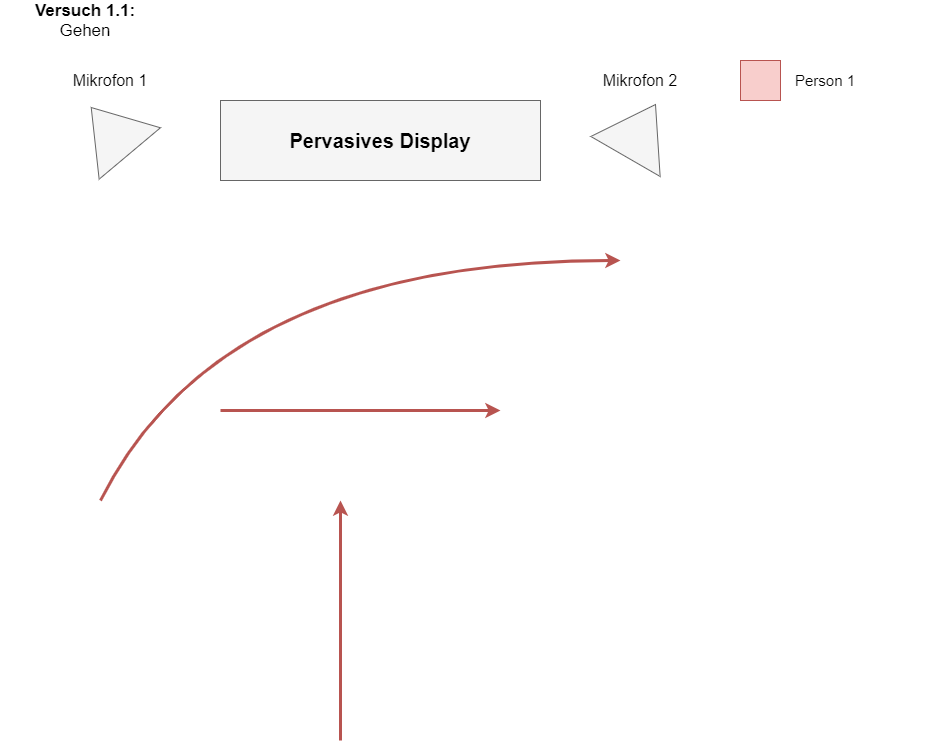
\includegraphics[width=\textwidth]{images/Versuch 1.1.PNG}
		\caption{Messung mit Gehen (eine Person)}
		\label{versuch1.1}
	\end{center}
\end{figure}
 


Die Pfeile auf der Abbildung \ref{versuch1.1} stellen die drei Routen dar, die eine einzelne Versuchsperson gehen wird. Durch die unterschiedlichen Wege entsteht automatisch ein variabler Abstand zu den Mikrofonen, was gleichzeitig eine realitätsnähere Situation abbildet. Die Versuchsperson geht zunächst von links aus in einem Bogen nach rechts auf den Bildschirm zu. Im Anschluss geht sie geradeaus, orthogonal zum Bildschirm, auf den Bildschirm zu und zuletzt läuft die Versuchsperson parallel zum Bildschirm geradeaus am Bildschirm vorbei. Für ein optimiertes Ergebnis wird jeder Weg wird mehrmals (fünf Mal) aufgezeichnet. Dies gilt auch für die nachfolgenden Versuche. Mit den Audiospuren des Versuchs mit einer Person besteht nun eine Grundlage für den späteren Vergleich.

Nachdem die Wege von einer Versuchsperson aufgezeichnet wurden, erfolgt eine ähnliche Durchführung mit zwei Personen. Die folgende Abbildung \ref{versuch1.2} soll die Versuchsdurchführung deutlicher zeigen.

 
\begin{figure}[H]
	\begin{center}
		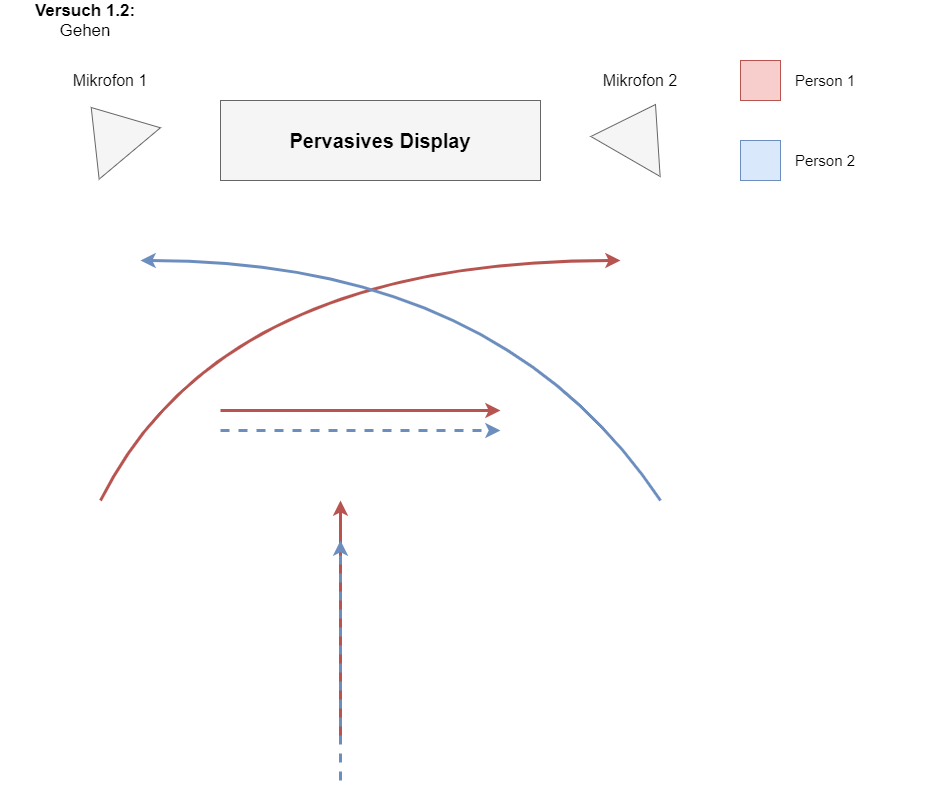
\includegraphics[width=\textwidth]{images/Versuch 1.2.PNG}
		\caption{Messung mit Gehen}
	\label{versuch1.2}
	\end{center}
\end{figure}

Analog zur Durchführung mit einer Person gehen hier zwei Personen die gleichen Wege. Die gestrichelte Darstellung der blauen Routen der zweiten Person stellt die Verdeckung dieser Person dar. Zu Beginn gehen die beiden Versuchspersonen jeweils ausgehend von links und rechts in einem Bogen auf den Bildschirm zu. Hierbei wird eine der Personen nur für einen kurzen Moment beim Kreuzen der Wege verdeckt. Diese kann aber auf Grund der unterschiedlichen Startpunkte auch durch Videoaufzeichnungen erkannt werden. Allerdings sollte die Audiospur trotzdem hilfreich sein, um Unterschiede zu Audiospuren zu erkennen, bei denen sich eine andere Anzahl von Personen vor dem Bildschirm bewegen. Im Anschluss gehen beide Personen hintereinander geradeaus auf den Bildschirm zu. Dabei ist eine Person verdeckt. Auch bei dem parallelen Vorbeilaufen zum Bildschirm wird eine der beiden Personen verdeckt, da sie in unserem Fall mit gleicher Geschwindigkeit nebeneinander laufen. 

Weiterhin möchten wir schauen, wie sich die Audiospuren ändern wenn sich drei Personen vor dem Bildschirm bewegen. Wie auch in den vorherigen zwei Versuchen nehmen wir keine Veränderung an den Wegen der Personen vor, damit wir einen optimalen Vergleich ziehen können. 

\begin{figure}[H]
	\begin{center}
		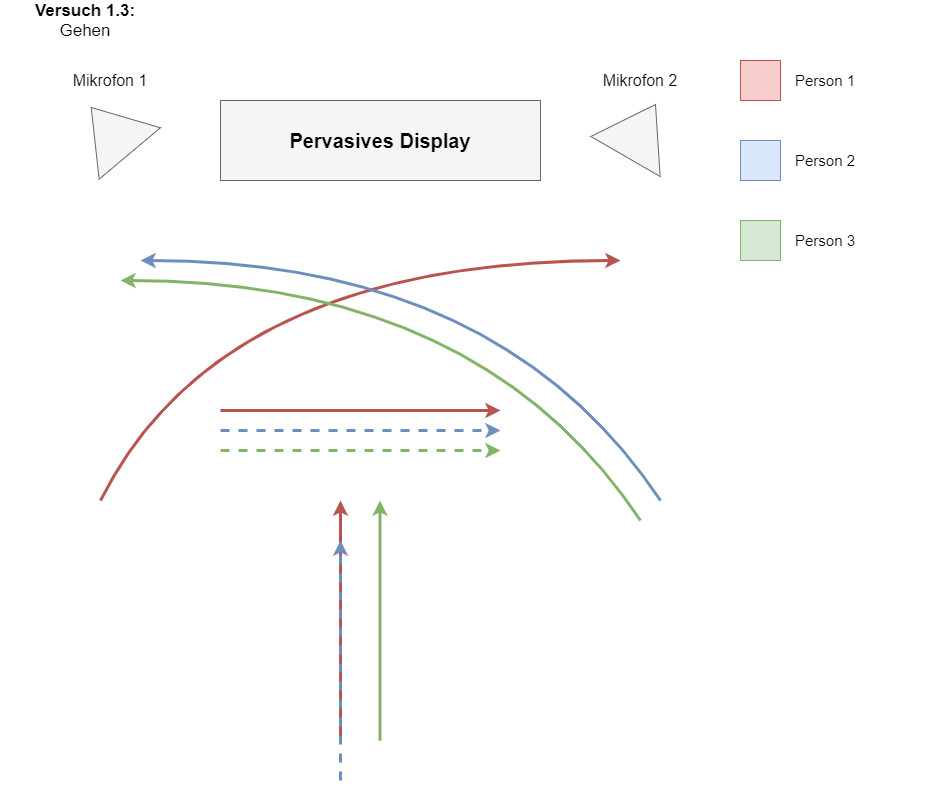
\includegraphics[width=\textwidth]{images/Versuch 1.3.PNG}
		\caption{Messung mit Gehen}
	\label{versuch1.3}
	\end{center}
\end{figure}

Im ersten Durchlauf starten zwei Versuchspersonen von links und eine dritte Versuchsperson von rechts. Auch hier kann für den Moment, in dem sich die Wege kreuzen eine oder auch zwei Personen verdeckt werden. Wie bereits beschrieben wurde kommt es aber bei dieser Situation auf Grund der unterschiedlichen Startpunkte mit Hilfe von Videoaufzeichnungen nicht vor, dass Personen nicht erkannt werden. Anders ist dies, wenn die drei Versuchspersonen geradeaus auf den Bildschirm zulaufen. In Abbildung \ref{versuch1.3} ist zu erkennen, dass zwei Personen nebeneinander gerade auf den Bildschirm zugehen. Im Schatten der beiden Personen läuft eine dritte Person, die von einer der beiden anderen Personen verdeckt wird. Auch beim parallelen Vorbeigehen der drei Versuchspersonen entsteht die Verdeckung von Personen. Da wir uns in dieser Versuchsreihe auf das Erkennen von visuell verdeckten Personen fokussieren, gehen die drei Personen in gleicher Geschwindigkeit am Bildschirm vorbei. Somit sind in diesem Fall sogar zwei Personen verdeckt. 

\subsection{Versuch Geschwindigkeit}

In der zweiten Versuchsreihe werden wir eine Versuchsperson in unterschiedlicher Geschwindigkeit am Bildschirm vorbeilaufen lassen. Die folgende Abbildung \ref{versuch2} soll die Versuchsdurchführung verdeutlichen. 

 
\begin{figure}[H]
	\begin{center}
		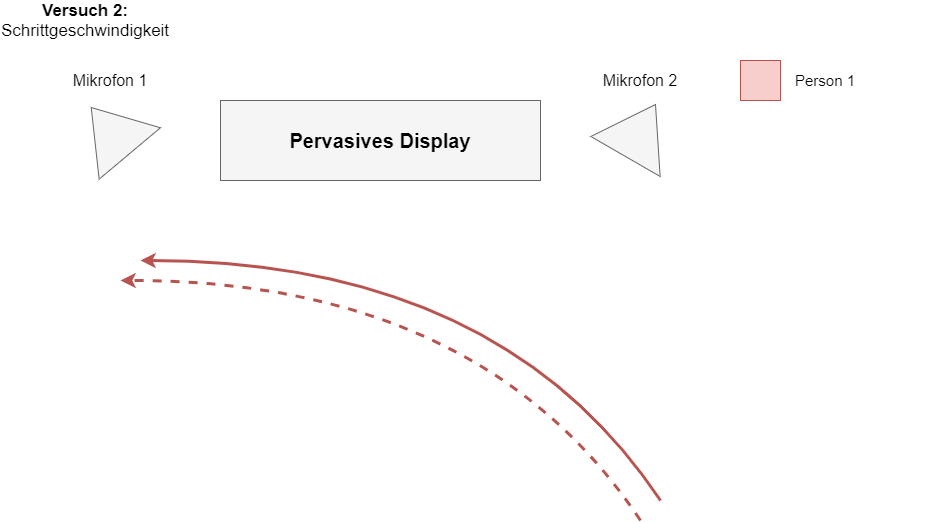
\includegraphics[width=\textwidth]{images/Versuch 2.PNG}
		\caption{Messung mit Schrittgeschwindigkeit}
	\label{versuch2}
	\end{center}
\end{figure}


Die Versuchsperson geht zunächst von links aus in einem Bogen auf den Bildschirm zu. Im weiteren Durchlauf läuft die Person dieselbe Strecke, allerdings schneller als zuvor. In diesem Versuch spielt der Weg, den die Person zurück legt keine große Rolle. Wichtig ist hierbei, dass bei beiden Geschwindigkeiten der Weg derselbe ist. So können die Audiospuren optimal miteinander verglichen werden und ein eindeutiges Ergebnis erwartet werden.

\subsection{Versuch Geräuschkulisse}

In der ersten Versuchsreihe (Abbildungen \ref{versuch1.1} bis \ref{versuch1.3}) haben wir bereits unterschiedliche Szenarien mit unterschiedlicher Anzahl von Versuchspersonen aufgenommen. Dabei gab es bisher keine beabsichtigten Geräusche im Hintergrund. Um die Versuchsumgebung realitätsnäher zu gestalten und im Nachhinein mögliche Fehler bei der Erkennung von Personen mit Audioaufzeichnungen vermeiden zu können, werden wir in dieser Versuchsreihe eine Geräuschkulisse hinzufügen. Hierbei stellen wir zwei unterschiedliche Arten von Geräuschen im Hintergrund dar. Zunächst Gespräche im Hintergrund und darauffolgend eine sich im Hintergrund bewegende Person.

Im ersten Versuchsdurchlauf werden wir nur eine Person mit Geräuschkulisse aufnehmen. Dies dient später wieder zum direkten Vergleich mit mehreren Personen. Mithilfe der folgenden Abbildung \ref{versuch3.1} soll der Versuchsablauf genauer beschrieben werden.

 
\begin{figure}[H]
	\begin{center}
		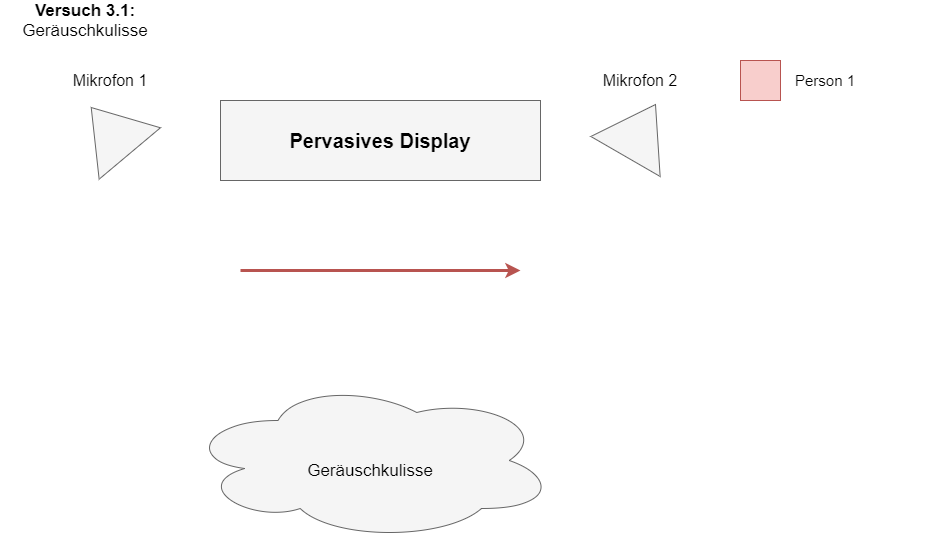
\includegraphics[width=\textwidth]{images/Versuch 3.1.PNG}
		\caption{Messung mit Geräuschkulisse}
	\label{versuch3.1}
	\end{center}
\end{figure}

Ähnlich wie bei den vorherigen Versuchsreihen läuft eine Versuchsperson parallel zum Bildschirm gerade aus an ihm vorbei. Die in Abbildung \ref{versuch3.1} dargestellte „Blase“ stellt die Geräuschkulisse dar. Während die Versuchsperson an dem Bildschirm vorbei läuft unterhalten sich im Hintergrund zwei Personen. In der nächsten Abbildung \ref{versuch3.2} ist dieser Versuch mit zwei Personen vor dem Bildschirm bildlich dargestellt.

 
\begin{figure}[H]
	\begin{center}
		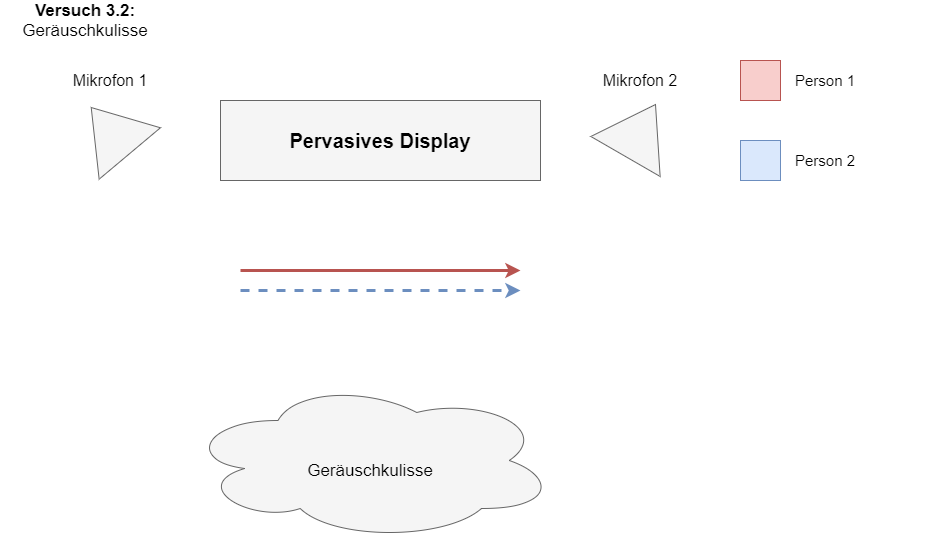
\includegraphics[width=\textwidth]{images/Versuch 3.2.PNG}
		\caption{Messung mit Geräuschkulisse}
	\label{versuch3.2}
	\end{center}
\end{figure}

Die oben aufgeführte Abbildung \ref{versuch3.2} zeigt wie zwei Personen parallel zum Bildschirm in gleicher Geschwindigkeit am Bildschirm vorbei gehen. Wie im vorherigen Versuch befindet sich im Hintergrund eine Geräuschkulisse in Form eines Gesprächs. Bei diesem Versuch entsteht eine visuelle Verdeckung einer Person. Mit Hilfe der Aufzeichnungen soll erkannt werden, ob die verdeckte Person trotz Gespräch im Hintergrund durch die Audiospur erkannt wird. 

In einem weiteren Versuchsdurchlauf haben wir die gleichen Szenarien wie in Abbildung \ref{versuch3.1} und \ref{versuch3.2} aufgenommen. Allerdings dieses Mal mit einer anderen Geräuschkulisse. Wie es auch in der Realität häufig vorkommt befinden sich bei diesem Versuch weitere bewegende Personen im Hintergrund. Auch hier haben wir eine und im Anschluss zwei Personen parallel zum Bildschirm am Bildschirm vorbeilaufen lassen. Wir wollen damit untersuchen, ob trotz bewegender Personen im Hintergrund, die Anzahl an Personen vor dem Bildschirm mit Hilfe von Audioaufzeichnungen erkannt werden kann.
